%%%%%%%%%%%%%%%%%%%%%%%%%%%%%%%%%%%%%%%%%%%%%%%%%%%%%%%%%
\section{Scenario}\label{sec:scenario}

Most competition tests take place in the \RoboCup\AtHome\Arena, but some tests may take place outside, in a previously unknown public place.
In this section, the \Arena{} and its contents are described, in particular the furnishing and other information that is common between tests and leagues.

\subsection{RoboCup@Home Arena}

The \RoboCup\AtHome\Arena{} is a realistic home setting (an apartment) consisting of inter-connected rooms.
The minimal configuration consists of:
\begin{itemize}
	\item a bedroom,
	\item a dining room,
	\item a living room, and
	\item a kitchen
\end{itemize}
There is usually one \Arena{} per league.
Depending on the local organization, there may also be multiple \Arena{}s that may be different from each other, and a robot must be prepared to perform any task in any \Arena{}.

The arena is arranged and decorated to resemble a typical apartment in the hosting country, including all necessities and decorations one can expect to find in a \emph{normal} home.
Note that what is considered \emph{normal} may vary greatly based on the culture and location where \RoboCup{} is hosted.
Decorations may include, but are not limited to, plants, mirrors, paintings, posters, plates, picture frames, wall clocks, candles with holders, and books.

\subsection{Walls, Doors, and Floor}\label{rule:scenario_walls}

The indoor home setting will be surrounded by high and low \Term{walls}{Arena walls}, which are built up using standard fair construction material.

\begin{enumerate}
	\item \textbf{Walls:} Walls are fixed and cannot be modified during the competition. The minimum wall height is \SI{60}{\centi\meter}; a maximum height is not specified, but must allow the audience to watch the competition.
	\item \textbf{Doors:} Inside the \Arena{}, rooms are connected by doors (at least one). All doors have handles, not knobs, and can be closed at any time; it is thus expected that robots are either able to open them or find a plan around them. All doors must meet minimum accessibility requirements but they should try to meet the recommended accessibility width of \SI{915}{\milli\meter}.
	\item \textbf{Floor:} The floor and doorways of the \Arena{} are even, so there are no significant steps or stairways; however, minor unevenness, such as carpets, transitions in floor covering between different areas, and minor gaps (especially at doorways) can be expected.
	\item \textbf{Appearance:} The floor and walls are mostly monochromatic, but may contain textures, such as a carpet on the floor, or a poster or picture on the wall.
\end{enumerate}


\subsection{Furniture}\label{rule:scenario_furniture}

The \Arena{} is furnished with typical objects common for the host country.
The minimal configuration consists of:
\begin{itemize}
	\item a bed,
	\item a couch,
	\item a small table,
	\item a small dinner table with two chairs,
	\item two trash bins,
	\item an open cupboard or a small table with a television and remote control,
	\item a chest of drawers,
	\item a high cabinet with doors
	\item a bookcase, and
	\item a coat rack
\end{itemize}
The \Arena{}'s kitchen has:
\begin{itemize}
	\item a dishwasher,
	\item a microwave,
	\item a sink, and
	\item a refrigerator (with some cans and plastic bottles inside)
\end{itemize}
A typical \Arena{} setup is shown in~\reffig{fig:scenario_arena}.
\begin{figure}[tbp]
	\centering
	\subfloat[Typical Arena]{\label{fig:scenario_arena}\includegraphics[height=46mm]{images/typical_arena.jpg}}
	\subfloat[Typical objects]{\label{fig:scenario_objects}\includegraphics[height=46mm]{images/typical_objects.jpg}}
	\caption{An example of a \RoboCup\AtHome{} scenario}\label{fig:arena}
\end{figure}

\subsubsection{Chest of drawers}

The Chest has at least two drawers that are between \SI{90}{\centi\meter} and \SI{120}{\centi\meter} from floor level. The drawers require U-shaped handles.

\subsubsection{High Cabinet}

The Cabinet can be any shelf-like furniture in which objects can be placed, such that the minimum distance between shelves is \SI{30}{\centi\meter}. The Cabinet needs two side by side doors blocking the access to at least the lower three of the shelves. The doors require U-shaped handles.

\subsubsection{Fridge}

At least one powered and functioning fridge is required in the \Arena.
The fridge must not be smaller than \SI{120}{\centi\meter}.

\subsection{Changes to the \Arena}\label{rule:scenario_changes}

Since robots should be able to function in the real world, the \Arena{} is not fixed and might change without further notice.
\begin{enumerate}
	\item \textbf{Major changes:}
	Any furniture (at a \PredefinedLocation{} or not) that cannot be expected to be fully static in an everyday environment might be moved slightly between tests.
	In particular, furniture will not change rooms or move drastically inside a room, but a couch or table may be slightly rotated or moved; fixed locations for such furniture items should not be assumed.
	Walls will stay in place and rooms will not change function.
	Passages might be blocked.
	\item \textbf{Minor Changes:} Slightly moved chairs, slightly closed doors, or anything similar cannot be avoided and might happen at any time, even during a test.
\end{enumerate}


%%%%%%%%%%%%%%%%%%%%%%%%%%%%%%%%%%%%%%%%%%%%%%%%%%%%%%%%%%%%%%%%%%
%
% Objects section.
%
% Revisited by Mauricio Matamoros for 2015
%
%%%%%%%%%%%%%%%%%%%%%%%%%%%%%%%%%%%%%%%%%%%%%%%%%%%%%%%%%%%%%%%%%%
\def\NumObjects{30\ }
\def\NumLocations{20\ }
\def\NumNames{20\ }

\subsection{Objects}\label{rule:scenario_objects}

Some tests in the RoboCup@Home league involve recognizing and manipulating objects (see Figure~\reffig{fig:scenario_objects}).
The TC will compile a list of at least \NumObjects{} objects for this purpose; the list will contain a picture of the each object, as well as its official name and \ObjectCategory{} (for instance, an \textit{Apple} belongs to the \textit{Fruits} category).
Most objects are likely to be lightweight and easy to grasp with one hand.
Every \ObjectCategory{} has an assigned \PredefinedLocation, where objects of that category can usually be found during tests (for example, an \textit{Fruits} can be found on the \textit{Kitchen Table}); assignments are announced during the \SetupDays{} (see~\refsec{chap:setup_and_preparation}).

Objects are provided at the competition for training.
Teams may keep at most five training objects at a time and for at most one hour.
Modifying the training objects is not allowed.

Two types of objects are used in the tasks:
\begin{enumerate}
	\item \textbf{\KnownObjects{}:} Objects previously known to the robot, divided into:
	\begin{enumerate}
		\item \textbf{\ConsistentObjects{}:} Objects whose image appears in the list of objects.
		\item \textbf{\SimilarObjects{}:} Objects whose image is not present in the list of objects, but look similar enough to one of them that a person would consider them the same kind of object. For example, an apple whose color is different from the apple in the list of objects, or a piece of cloth with a different pattern.
		\item \textbf{\StandardObjects{}:} Objects chosen from the \YCBData{}.\footnote{\url{http://www.ycbbenchmarks.com/object-set/}} They are published 6 months in advance on the \RoboCup\AtHome{} website\footnote{\url{https://athome.robocup.org/standard-objects}}, so that they can be aquired and trained beforehand.
	\end{enumerate}
	\item \textbf{\UnknownObjects{}:} Any other object that is not in the object list but can be grasped or handled (e.g., \Arena{} decorations).
\end{enumerate}

The minimal configuration of \KnownObjects{} consists of:
\begin{itemize}
	\item \textbf{\iterm{Tableware}:} Dish, bowl, cup (or mug), and napkin (see Figure~\ref{fig:scenario_container_bowl}).
	\item \textbf{\iterm{Cutlery}:} Fork, knife, and spoon.
	\item \textbf{\iterm{Trash Bags}:} Big plastic trash bags, preferably with a handle.
	\item \textbf{\iterm{Bags}:} Lightweight and with stiff, vertical handles (see Figure~\ref{fig:scenario_container_bag}).
	\item \textbf{\iterm{Dry Food Container}:} Dry food containers (see Figure~\ref{fig:scenario_container_dry}).
	\item \textbf{\iterm{Disks or books}:} A set of discs (LP, CD, DVD, or BluRay) or books.
	\item \textbf{\iterm{Coat rack}:} A rack or pole to hang coats and other clothes.
	\item \textbf{\iterm{Trays}:} A transport object such as a tray or basket, intended for bimanual manipulation (see Figure~\ref{fig:scenario_container_tray}).
	\item \textbf{\iterm{Pourable}:} An object whose content can be poured (such as a cereal box).
	\item \textbf{\iterm{Heavy object}:} Weight between 1.0kg and 1.5kg.
	\item \textbf{\iterm{Tiny object}:} A lightweight object that is not bigger than \SI{5}{\centi\meter} (such as paper, a teabag, or a pen).
	\item \textbf{\iterm{Fragile object}:} An easy-to-break object, (such as a chocolate egg).
	\item \textbf{\iterm{Deformable object}:} A flexible object that may take different shapes (such as cloth).
	\item \textbf{\iterm{Garbage bag}:} A garbage bag that can be tied.
\end{itemize}

\begin{figure}[H]
	\centering
	\subfloat[Cereal bowls]{
		\includegraphics[width=0.33\textwidth]{images/container_bowl.png}\label{fig:scenario_container_bowl}}
	\subfloat[Bright-colored paper bags]{
		\includegraphics[width=0.33\textwidth]{images/container_paper_bag.png}\label{fig:scenario_container_bag}}
	\subfloat[Serving tray]{
		\includegraphics[width=0.33\textwidth]{images/container_tray.png}\label{fig:scenario_container_tray}}
	\subfloat[Dry food Container]{
		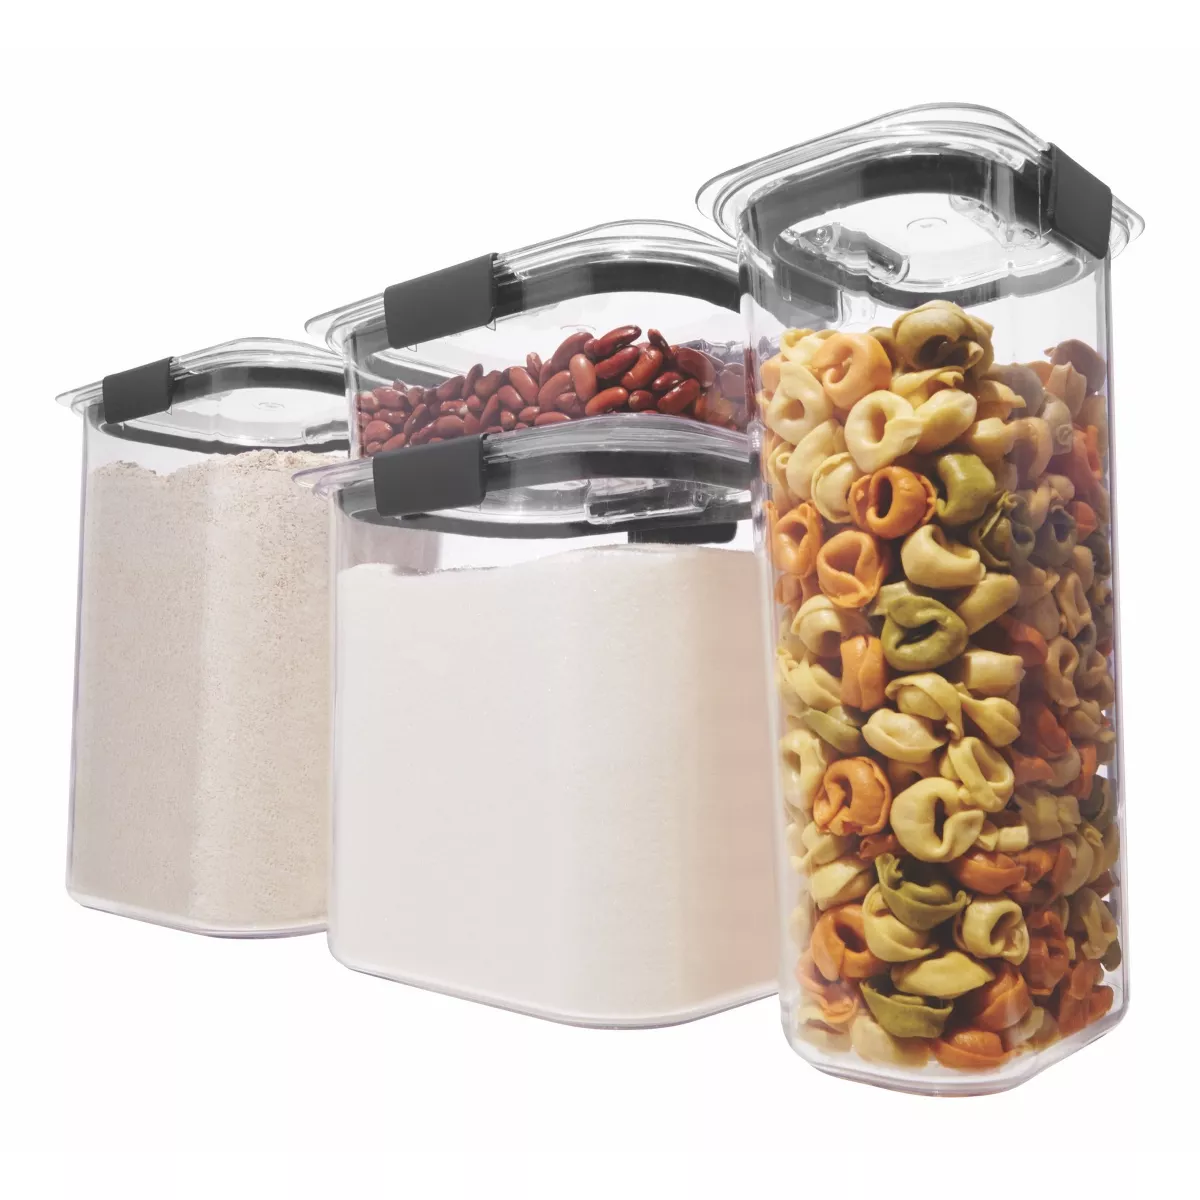
\includegraphics[width=0.33\textwidth]{images/container_dry.png}\label{fig:scenario_container_dry}}
	\caption{Example of object containers}
	\label{fig:scenario_containers}
\end{figure}

During the competition, objects can be requested based on their \ObjectCategory{}, physical attributes, or a combination of both.
Relevant attributes to be used are:
\begin{itemize}
	\item Color (such as red, blue, black with white dots, etc.).
	\item Relative estimated size (smallest, largest, big one, etc.).
	\item Relative estimated weight (lightest, heaviest).
	\item Relative position (left of, rightmost, etc.).
	\item Object description (is fragile, is a container, can be poured, requires two hands, etc.).
\end{itemize}

\noindent\textbf{Remark:} Measurements are estimations and based on common sense. It is OK for robots to consider similar objects to be about the same size or weight.

%%%%%%%%%%%%%%%%%%%%%%%%%%%%%%%%%%%%%%%%%%%%%%%%%%%%%%%%%%%%%%%%%%
%
% Predefined locations section.
%
%%%%%%%%%%%%%%%%%%%%%%%%%%%%%%%%%%%%%%%%%%%%%%%%%%%%%%%%%%%%%%%%%%

\subsection{Predefined Rooms and Locations}\label{rule:scenario_locations}

Some tests in the RoboCup@Home league involve a \PredefinedLocation{} where people or objects can be found.
There will also be at least two \Term{doors}{Arena doors}, named an \Entrance{} and an \Exit, which lead in and out of the \Arena{}, respectively.
Room names, predefined locations, and location classes are announced during the \SetupDays{} (see~\refsec{chap:setup_and_preparation}).

\subsection{Predefined Person Names}\label{rule:scenario_names}

Some tests in the RoboCup@Home league involve memorizing a person's name.
All people in the \Arena{} have an assigned \PredefinedName{} chosen by the TC.
The list of names contains \SI{25}{\percent} male, \SI{25}{\percent} female, and \SI{50}{\percent} gender-neutral names taken from the list of most commonly used names in the United States.
Predefined names are announced during the \SetupDays{} (see~\refsec{chap:setup_and_preparation}).

\subsection{Wireless network}\label{rule:scenario_wifi}

For wireless communication, an \ArenaNetwork{} is provided.
The actual infrastructure depends on the local organization.
Reliability and performance of the network is not guaranteed; robots are expected to be able to run without a wireless network.

The following rules apply:
\begin{itemize}
	\item Only the \ArenaNetwork{} can be used during tests.
	\item Only the active team in a task is allowed to use the \ArenaNetwork.
	\item The \ArenaNetwork{} provides one Virtual Local Area Network (VLANs) per team.
	\item Each VLAN is most likely to have its own SSID/password.
	\item VLAN traffic is separated from any other team and is routed to the team's network cable in the team area.
	\item Each VLAN is also connected to the Internet.
\end{itemize}

Teams broadcasting unauthorized (aka rogue) wireless networks will be disqualified from the competition and their devices may be temporarily confiscated by the OC, this includes smartphones and concealed SSIDs.
It is thus advised to verify your devices for any breaches of this nature.


% Local Variables:
% TeX-master: "../Rulebook"
% End:
